\documentclass[a4paper,11pt]{article}
\usepackage[left=.8in, right=.8in, top=.6in, bottom=.6in]{geometry}
\usepackage{enumitem}
\usepackage{titlesec}
\usepackage{parskip}
\usepackage{xcolor}
\usepackage{fontawesome5}
\usepackage[hidelinks]{hyperref}
\usepackage{graphicx}
\usepackage{multicol}
\usepackage[color=green]{todonotes}
% Run with XeLaTeX!

% Define el color verde olivo
\definecolor{verdeolivo}{RGB}{85,107,47} % Puedes ajustar estos valores según tus preferencias
\definecolor{glauco}{RGB}{91, 127, 197}

\titleformat{\section}{\large\bfseries\color{verdeolivo}}{}{0em}{}[\titlerule]
\titleformat{\subsection}[runin]{\bfseries\color{verdeolivo}}{}{0em}{}[:]

\begin{document}

\pagestyle{empty}



%\section*{\faIcon{address-card} Contact Information}
\begin{center}
    \textbf{\Huge Greta Coraglia} \\
%    \vspace{2mm}
%    \faIcon{briefcase} Quality Engineer
\vspace{2mm}
    \faIcon{link} \url{https://etagreta.github.io/}
	\qquad
    \faIcon{envelope} \href{mailto:coraglia.eta@gmail.com}{coraglia.eta@gmail.com}
	\qquad
    \faIcon{map-marker-alt} 09/04/1994, Italy
\end{center}


\space
\vspace{.5cm}

\begin{minipage}{0.58\textwidth}
\section*{\faIcon{user} Professional profile}
I am a mathematician with experience in research and interdisciplinary collaboration, passionate about tackling complex problems from multiple perspectives. I am experienced in teaching, public speaking, and communicating complex ideas with clarity, with a focus on making AI accessible and empowering for diverse audiences. I am active in civic life and motivated by social impact. I am calm under pressure, proactive, and team-oriented, and I cherish in connecting people and ideas to deliver pragmatic solutions.
\end{minipage}\hfill
\begin{minipage}{0.35\textwidth}
    \begin{center}
    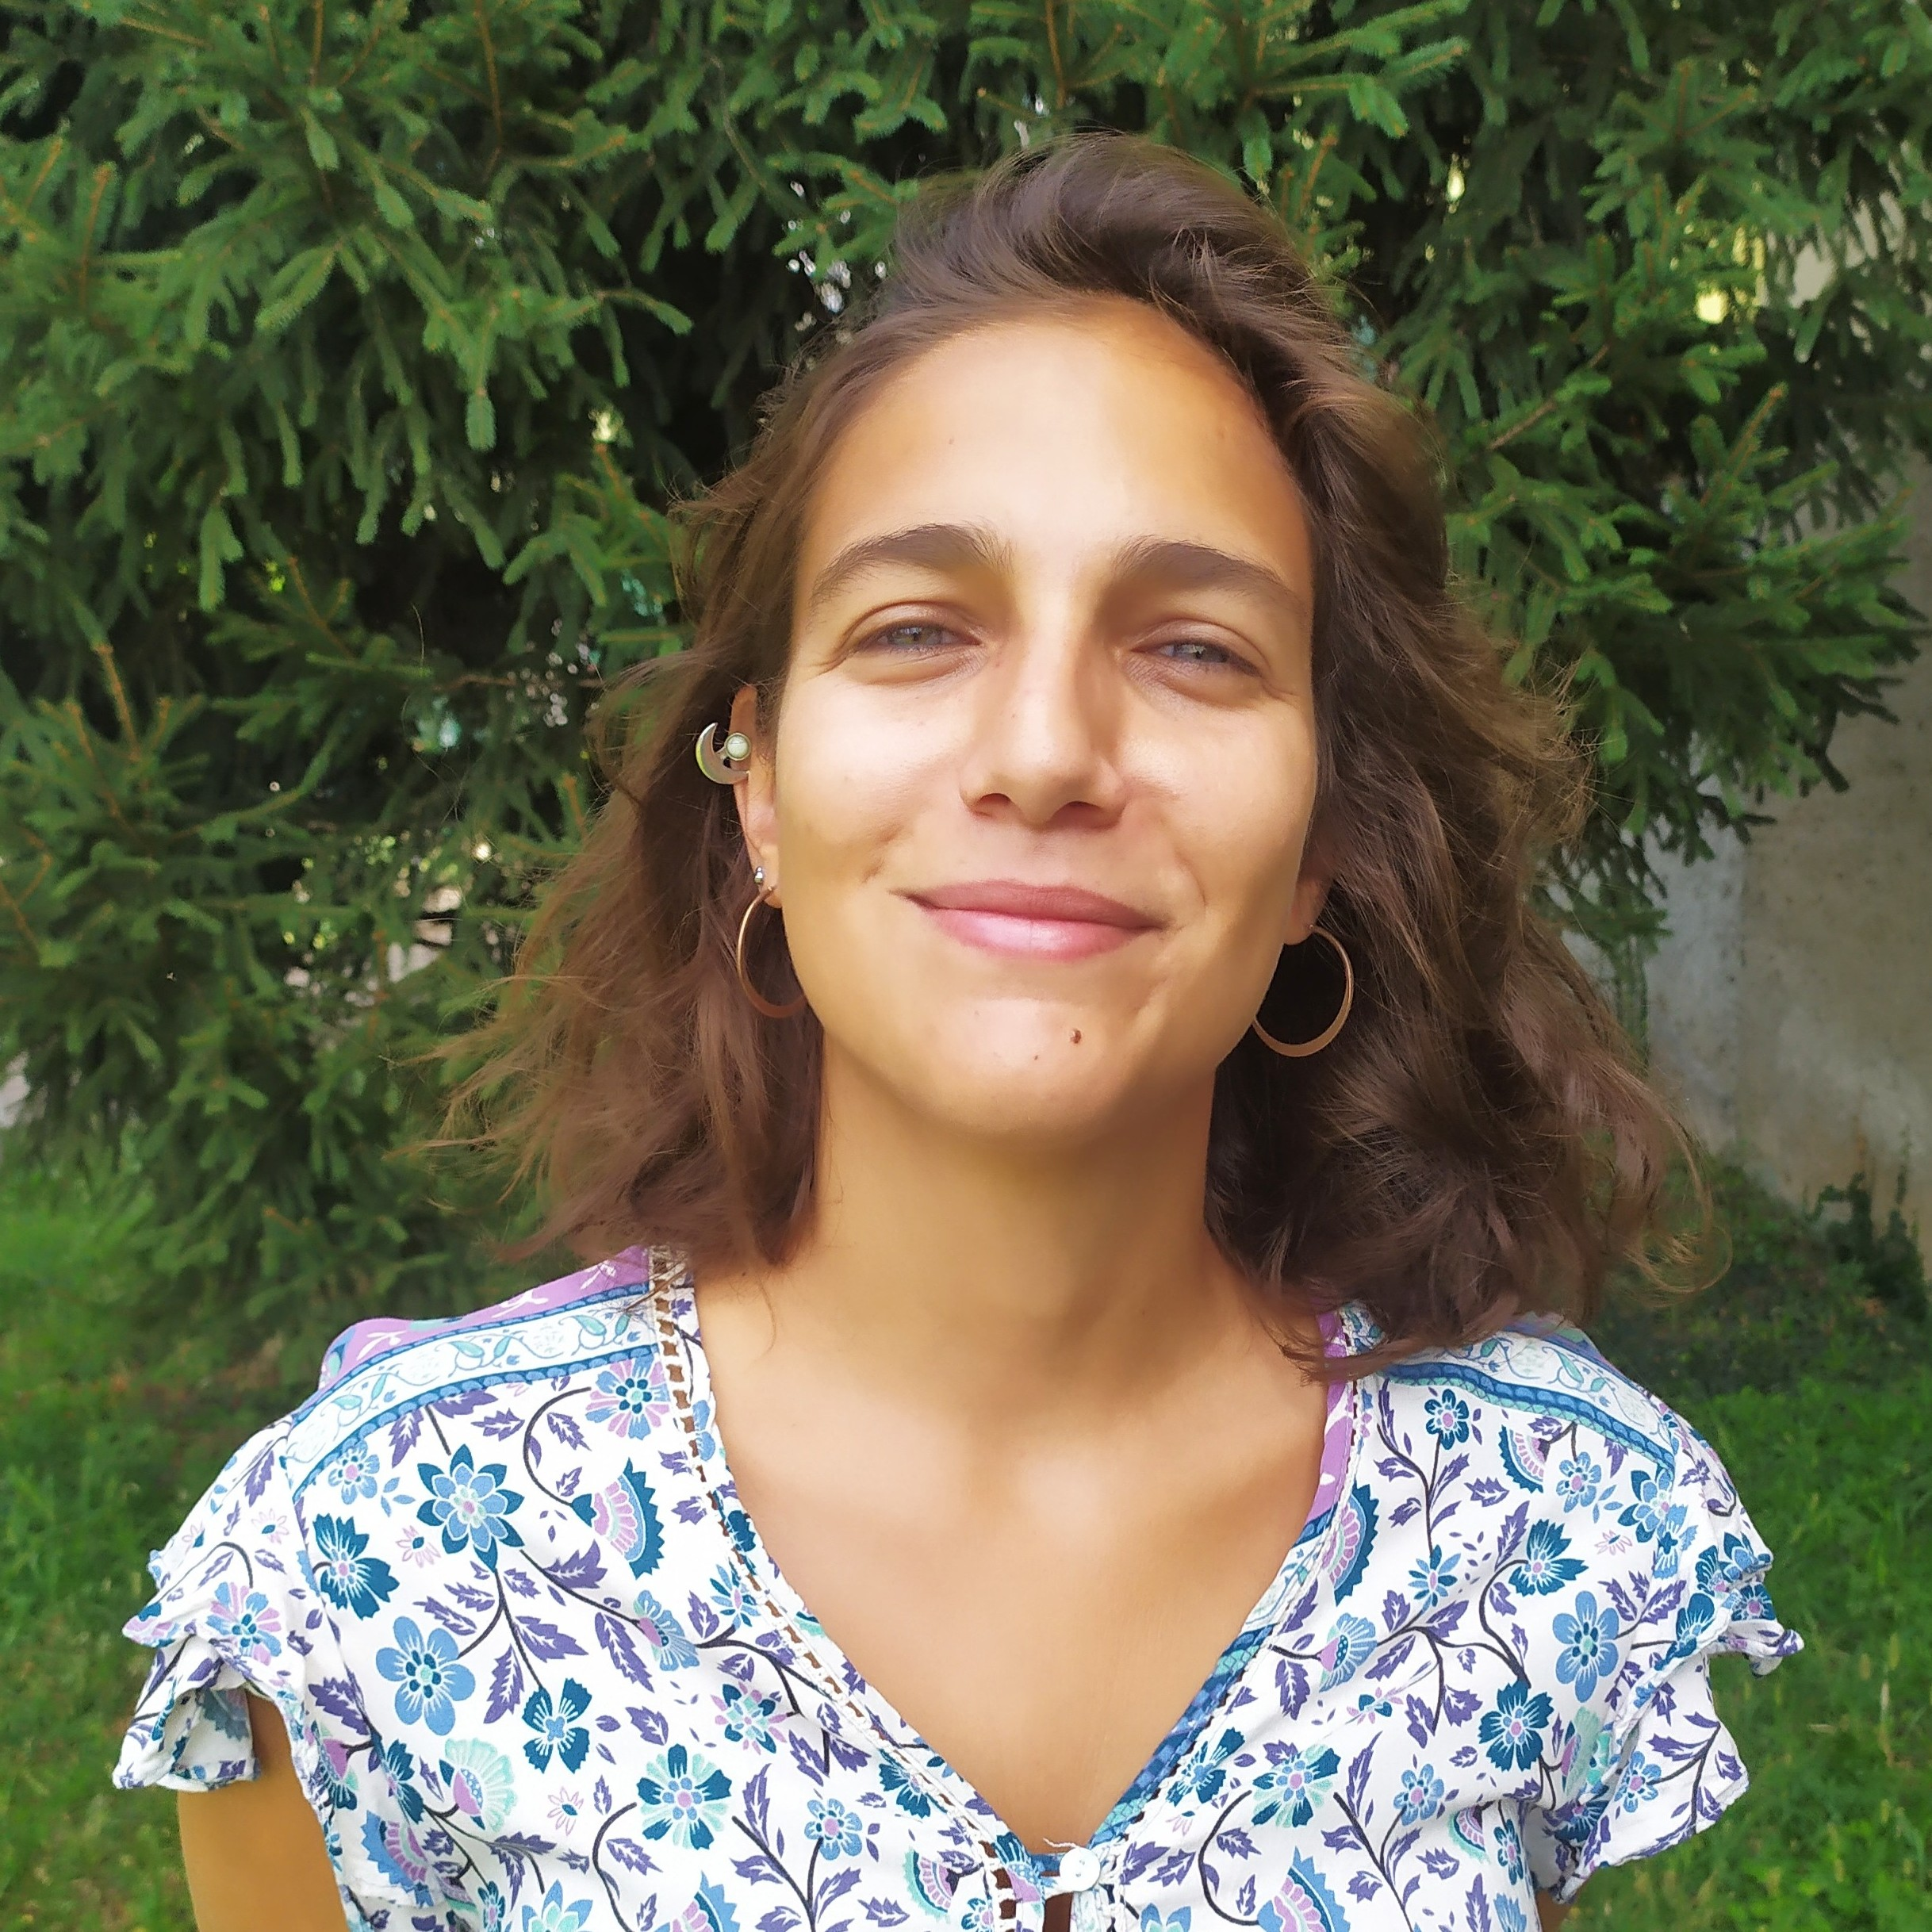
\includegraphics[width=.9\textwidth]{coraglia.jpg}
	\end{center}
\end{minipage}


\section*{\faIcon{building} Relevant work experience}

\subsection*{MIRAI Srl \hfill Mar 2024 - present}
\textit{Founder, research associate} \\
Co-founded a start-up in collaboration with industry experts to help public and private organizations achieve regulatory compliance while upholding the highest standards of transparency and fairness. I moved the research in the background of different projects, spanning from RAG evaluation to assessment of ML classification algorithms.

\subsection*{University of Pavia \hfill Mar 2025 - present}
\textit{Adjunct professor in Logics for AI} \\
Lectured for the Logics for Practical Reasoning and AI course in the joint Bachelor’s program in Artificial Intelligence (UniPv–UniMi–UniMiB). This role expanded my expertise in causal graphs and honed my public speaking, communication, and organizational abilities.

\subsection*{Segrate City Council \hfill Sep 2020 - present}
\textit{Majority chief whip} \\
Co-organized a civic movement and was elected to my city’s council on a civic list. Currently serving as chief whip of the largest council group and as vice-president of the council. Responsibilities include coordinating council activities on key policy issues, drafting and advancing legislative proposals, negotiating with institutional offices and stakeholders, and organizing public events to inform and actively engage citizens in shaping and implementing public policy.

\subsection*{University of Milan \hfill Mar 2023 - July 2025}
\textit{Postdoctoral researcher} \\
Conducted research in the BRIO (Bias, Risk, and Opacity in AI) project, advancing formal methods to assess AI fairness and risk. I co-developed open-source tools in partnership with private companies for real-world applications, such as to credit scoring. I benefitted from working within a multidisciplinary team, combining strong technical problem-solving with effective cross-sector communication.

\subsection*{University of Genoa \hfill Nov 2019 - Aug 2023}
\textit{Doctoral candidate in Mathematics}\\
Worked for a Ph.D. in Mathematics with specialization in logic, category theory, type theory, and theoretical computer science. I developed a strong foundation in rigorous problem-solving and abstract reasoning, with practical applications to formal system design, programming language theory, and algorithmic thinking.

During this time, I also taught a Linear Algebra (Geometry) course to first-year Electronic Engineering students. That strengthened my ability to explain complex technical concepts clearly, while reinforcing my expertise in linear algebra with emphasis on its engineering applications in data modeling.

%\subsection*{University of Genoa \hfill 2020 - 2022}
%\textit{TA for Linear Algebra}\\
%Taught Linear Algebra (Geometry) course to first-year Electronic Engineering students, designing exercises and assessments. That strengthened my ability to explain complex technical concepts clearly, while reinforcing my expertise in linear algebra with emphasis on its engineering applications in data modeling.

\newpage

\section*{\faIcon{graduation-cap} Education}
\textbf{University of Genoa} \hfill \textit{Nov 2019 -- Aug 2023} \\
\textit{Ph.D. in Mathematics} \\
Thesis: ``Categorical structures for deduction'', supervisor: Prof. G. Rosolini \\
\textbf{Expertise:} logic, category theory, theoretical computer science, type theory 

\textbf{University of Milan} \hfill \textit{2017 -- 2019} \\
\textit{M.Sc. in Mathematics (with honors)} \\
Thesis: ``A categorical perspective on Heyting-valued sets'', sups: Profs. S. Ghilardi and G. Rosolini \\
\textbf{Expertise:} logic, category theory, fuzzy logic, automated reasoning, formal methods

\textbf{University of Milan} \hfill \textit{2013 -- 2017} \\
\textit{B.Sc. in Mathematics} \\
\textbf{Expertise:} algebra, linear algebra, geometry, logic, foundations of mathematics



%\section*{\faIcon{atom} Research projects}
%\subsection*{\href{https://arxiv.org/abs/2406.03292}{Risk assessment in credit scoring} \hfill 2023 - present}
%\textit{j/w BRIO@UniMi}\\
%Quantifying the risk inherent to opaque classification algorithms, with applications to credit scoring. In collaboration with companies operating in the private sector.
%
%\faIcon{angle-right}\, Submitted for publication.
%
%\subsection*{\href{https://ceur-ws.org/Vol-3615/paper4.pdf}{Bias detection for opaque AI systems} \hfill 2023}
%\textit{j/w BRIO@UniMi and Alkemy}\\
%Developing a fairness metric based on a typed $\lambda$-calculus for probabilistic programs.
%
%\faIcon{angle-right}\, Presented at 22nd International Conference of the Italian Association for Artificial Intelligence (AI*IA 2023). Published in the \emph{Proceedings of the 2nd Workshop on Bias, Ethical AI, Explainability and the role of Logic and Logic Programming}, 2023.
%
%\subsection*{\href{https://drops.dagstuhl.de/entities/document/10.4230/LIPIcs.TYPES.2023.3}{Categorical models of subtyping} \hfill 2023}
%\textit{j/w J. Emmenegger}\\
%Using categorical tools to infer desirable notions of subtyping (related coercive subtyping).
%
%\faIcon{angle-right}\, Accepted for TYPES 2023 (Jun 2023) and 108th PSSL (Sep 2023), presented in an invited talk at the LAMA Group at Université Savoie Mont Blanc (Nov 2023). Published in the \emph{Proceedings of TYPES 2023}, 2024.
%
%\subsection*{\href{https://arxiv.org/abs/2408.16581}{On the fibration of algebras} \hfill 2022 - 2024}
%\begin{flushright}
%\vspace{-.8em}
%\textit{j/w Castelnovo, Loregian, Martins-Ferreira, Ahman, Reimaa}
%\end{flushright}
%\vspace{-.5em}
%Studying algebraic properties of parametric endofunctors, co/monads, and their algebras. Using the theory of fibered categories to produce abstract results describing their behaviour.
%
%\faIcon{angle-right}\, Presented at an invited talk at HoTTEST (Mar 2024) and CATNIP (May 2024). Submitted for publication.
%
%\subsection*{\href{https://arxiv.org/abs/2403.03085}{A 2-dimensional analysis of context comprehension} \hfill 2022 - 2024}
%\textit{j/w J. Emmenegger}\\
%Extending set-based models for dependent types to cat-based models. Studying the inherently coalgebraic nature of context comprehension.
%
%\faIcon{angle-right}\, Presented at invited talks at HoTT/UF (Apr 2023), accepted for a talk at ItaCa Fest (May 2022). Accepted for publication in \emph{Theory and Applications of Categories}, 2024.
%
%\subsection*{Fuzzy type theory for opinion dynamics \hfill 2022 - present}
%\textit{j/w Adjoint School}\\
%Using enriched category theory to provide suitable syntax and semantics for a fuzzy type theory, with the perspective of applying it to (sheaf) opinion dynamics.
%
%\faIcon{angle-right}\, Presented as a poster at ACT 2023 (by S.J. O'Connor) and at the Logic Colloquium (Jun 2023). In preparation.
%
%\subsection*{\href{https://arxiv.org/abs/2111.09438}{Context, judgement, deduction} \hfill 2021 - 2022}
%\textit{j/w I. Di Liberti}\\
%Introducing judgemental theories and their calculi as a general framework to present and study deductive systems. Specifying to dependent type theory and natural deduction as special kinds of judgemental theories.
%
%\faIcon{angle-right}\, Accepted talk at Logic and higher structures at CIRM (Feb 2022) and TACL (Jun 2022), presented at an invited talk for the Compositional Systems and Methods group at TalTech. In publication.
%
%\section*{\faIcon{glasses} Para-academic activities}
%\textit{Organizing.} Contributed to the organization of Bias, Risk, Explainability and the role of Logic and Logic Programming (joint with AI*IA -- Bolzano, 2024), Effectiveness and Continuity in Categorical Logic (Genoa, Sep 2024), Logic Colloquium (Milan, Jun 2023), 2nd ItaCa Workshop (Genoa, Dec 2021).
%
%\textit{Chairing.} Sitting on the Scientific Committee for ItaCa (since spring of 2023), on the Program Committee for TYPES 2024 and for ACT 2024.
%
%\textit{Reviewing.} Reviewed for the American Mathematical Society and for the International Journal of Approximate Reasoning.
%
%\textit{Visiting.} Visited the Mathematics Department at the University of Aberdeen (May 2023), the Laboratoire de Mathématiques de l'Université Savoie Mont Blanc (Nov-Dec 2023), the Compositional Systems and Methods group at Tallinn's University of Technology (May 2022).
%
%\textit{Honors and awards.} Won the prize for Best Master's Thesis in Logic (2019) awarded by the Italian Logic Association (AILA). Won several research and travel grants: the Adjoint School participation (2022), a stay at CIRM Marseille (2022) for ``Logic and Higher Structures'' and ``Linear Logic Winter School'', travel to the Symposium on Compositional Structures (SYCO, 2019), and invitations as in the previous section.

\section*{\faIcon{glasses} Awards, certifications, and such}
\textit{Academic.} Won the prize for Best Master's Thesis in Logic (2019) awarded by the Italian Logic Association (AILA). Won several research and travel grants: the Adjoint School participation (2022) in Glasgow, a stay at CIRM Marseille (2022) for ``Logic and Higher Structures'' and ``Linear Logic Winter School'', travel to the Symposium on Compositional Structures (SYCO, 2019) in Leicester, and invitations to visit the Mathematics Department at the University of Aberdeen (May 2023), the Laboratoire de Mathématiques de l'Université Savoie Mont Blanc (Nov-Dec 2023), the Compositional Systems and Methods group at Tallinn's University of Technology (May 2022).

\textit{Linguistic.} British Council Aptis ESOL attested (January 2025) CEFR grade: C2.

\textit{Reasoning and numerical.} Successfully passed (June 2024) selection tests from the European Personnel Selection office highest grade: EPSO/CAST/P/17/2017 - Information and communication technology (FG IV).

%{\color{red}
%\textit{Machine learning.} Coursera Stanford....
%ML fundamentals and implementation: predictive tasks, classification problems, clustering.
%}

\section*{\faIcon{cogs} Technical tools}
Python, C, Git, tools for formal methods (SAT, SMT, Prolog, NuSMV).
	
\section*{\faIcon{user-friends} Social involvement}

%\textit{Politics.} I organized a small civic movement and got elected with a civic list to my city's council. I am
%currently chief whip of the largest group in the council and vice-president of the council itself.
%My job consists in organizing the council's work around the issues of our interest, in advancing legislative
%proposals, in meeting with relevant offices and stakeholders, and in organizing public events both to inform
%and engage citizens in defining and enforcing public policies.

\textit{Popularization.} I am a strong believer in the necessity of democratizing knowledge: during COVID with some friends we organized community seminars on YouTube, and I gave one on the concept of infinity; in 2020 with a colleague we participated in a high school programme teaching logic (syllogisms and Turing machines) to high-school students; with ItaCa, I helped organizing a YouTube course in category theory with specialists in the topic; I wrote about constructive mathematics in a dissemination journal; with some friends and colleagues we are organizing a public conference to demystify the narrative on AI, to acknowledge its benefits, and to encourage action.

%\textit{Volunteering.}

\textit{Translating etc (English).}  Translated two books and contributed to a community initiative preparing Italian subtitles for international works. Provided interpreting support for authors at an international book festival, facilitating communication across languages and cultures.

%\section*{\faIcon{leaf} Random}
%\todo[inline]{Traduzione?}

\vfill
\hfill\small\textit{Last updated: September 2025}

\end{document}